
\chapter{Analysis and High-Level Design}

It is the goal of this thesis to enable detection of sleep-related disorders with the aid of an Android device and low-cost sensors, and to further analyze and evaluate sleep- and breath-related patterns. We developed an application, called \textit{Nidra}, which attempts to collect, analyze, and share data collected from external sensors, all on a mobile device. Also, Nidra acts as a platform for modules to enrich the data, thus extending the functionality of the application.

The motivation behind this application is to provide an interface for patients to potentially run a self-diagnostic from home, and to aid researchers and doctors with analysis of sleep- and breathing-related illnesses (e.g., Obstructive Sleep Apnea). An overview of the Nidra application pipeline is found in Figure \ref{fig:parts}, beginning with data acquired from a sensor, and ending with the data in the Nidra application. As for now, Nidra consists of three main functionalities, each related to the requirements defined in the problem statement: 

\begin{enumerate}
    \item The application must provide an interface for the patient to (i) record physiological signals (e.g., breathing data); (ii) present the results; and (iii) share the results.
    \item The application must ensure that upon sensor disconnections, the connectivity is reinstated to minimize the data loss and its effects on the data analysis.
    \item The application must provide an interface for the developers to create modules that integrate with the application.
\end{enumerate}

This chapter will give a detailed look at the design of Nidra, including the tasks which constitute the structure of the application, the separate concerns in relation to the tasks, and the structure of the data in the application.

\section{Requirement Analysis}

\subsection{Stakeholders}
McGrath and Whitty \cite{stakeholderdefined} describe the term stakeholder as those persons or organizations that have, or claim an interest in the project. They distinguish stakeholders into four categories: (1) \textit{contributing (primary) stakeholders} participate in developing and sustaining the project; (2) \textit{observer (secondary) stakeholders} affect or influence the project;  (3) \textit{end-users (tertiary stakeholder)} interact and uses the output of the application; and (4) \textit{invested stakeholders} have control of the project. In Nidra, three stakeholders affect the application, and each is categorized respectively:
\begin{itemize}
    \item \verb|Patients| are identified as an end-user---they interact with the application.  
    \item \verb|Researchers/Doctors| are identified as an observer stakeholder---they might not use the application itself; however, they might use the data obtained from the patients' recordings for further analysis. Also, request functionality in the application.
    \item \verb|Developers| are identified as a contributor stakeholder---they maintain the application from bugs. Additionally, they can contribute to developing modules that extend the functionality of the application. 
\end{itemize}

\subsection{Resource Efficiency}
The application is designed for the use on a mobile device; modern mobile devices are empowered with multi-core processors, a sufficient amount of RAM, and a variety of sensors. However, the battery capacity is restrictive and based on usage. The device may only last for one day before a charge, due to the size of the battery capacity \cite{androidbattery}. The average battery capacity of a mobile device is approximately 2000 mAh on budget devices and approximately 3000 mAh on high-end devices \cite{androidbatteryavg}. The application should be able to run at least 7 hours without any power supply. Also, the device should be capable of handling various sensor connections simultaneously. Therefore, the application should be designed to be resource-efficient by utilizing the least amount of battery resources during a recording. Also, ensure a sufficient amount of power on the device before starting a recording session.  

\subsection{Security and Privacy}
The proposed use of the application is to monitor the sleeping patterns of a patient. The application manages and stores personal- and health-related data about the patient. As a precaution, the application should incorporate the CIA triad, which stresses data confidentiality, integrity, and availability \cite{cia}. Any unauthorized access to the data, data leaks and confidentiality should be appropriately managed on the device. Sharing the data across application or with researchers/doctors should be granted with the consent from the patient.  Besides, a mobile device can be connected to the Internet, which makes it vulnerable to attacks. Also, other installed application on the device can manipulate the access to the data. Therefore, revising the security policy defined by Android \cite{androidsecurity} should be incentivized. 

\section{High-Level Design}

\subsection{Task Analysis}
Task analysis is a methodology to facilitate the design of complex systems. Hierarchical task analysis (HTA) is an underlying technique that analyzes and decomposes complex tasks such as planning, diagnosis, and decision making into specific subtasks \cite{ta}. In Figure \ref{fig:hta_overview}, an illustration of the tasks of the application is presented. This section introduces these tasks, which are an integral part of the development of the application.

\begin{figure}
    \centering
    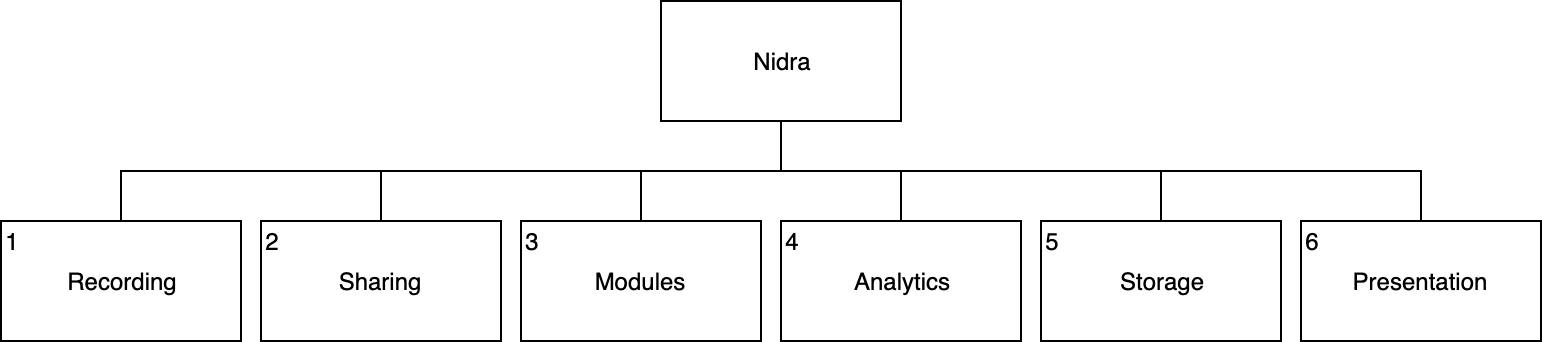
\includegraphics[scale=0.23]{images/TA.png}
    \caption{Recording}
    \label{fig:hta_overview}
\end{figure}

%\subsubsection{System Tasks}

\noindent\textbf{Recording}

\noindent A \textit{recording} is a process of collecting and storing physiological signals (e.g., breathing data) from sensors over an extended period (e.g., overnight). To enable a recording, we need to establish connections to available sensors, collect samples from the sensors, and store the samples on the device. A \textit{sensor} is a device that transforms analog signals from the real world into digital signals. The digital signals are transmittable over Link Layer technologies (e.g., BlueTooth), and the communication between a sensor and device occurs based on the protocols the sensor supports. A \textit{sample} is a single sensor reading containing data and metadata, such as time and the physiological data. During the recording session, ensuring that the sensors and the devices maintain connectivity such that the record contains meaningful data.  Once a recording session has terminated, a \textit{record} with metadata about the recording session is stored, alongside the samples.    

\noindent \textbf{Sharing}

\noindent Sharing is a mechanism to export and import records across applications. \textit{Exporting} consists of bundling one or more records with correlated samples into a transmittable format and transferring the bundled records over a media (e.g., mail). \textit{Importing}, on the other hand, consists of locating the bundled records on the device, parsing the content and storing it on the device. The sharing mechanism allows the patients to send their records to researchers/doctors.

\noindent \textbf{Module}

\noindent A \textit{module} is an independent application that is installed and launched in Nidra (hereafter: application), to provide extended functionality and data enrichment. A module does not necessarily interact with the application. However, it utilizes the data (e.g., records). For example, a module could be using the records to feed a machine-learning algorithm to predict obstructive sleep apnea. Installing a module is achieved by locating the module-application on the device, and storing the reference in the application. Due to limitations in Android, the module-application cannot be executed within the application. Therefore, the module-application is a standalone Android application. Furthermore, the development of the module-application is independent of the application. 

\noindent \textbf{Analytics}

\noindent Analytics is the visualization and interpretation of patterns in the records. The application facilitates the recording of breathing data, which enables the detection and analysis of sleep-related breathing disorder. There are various analytical methods, ranging from graphs to advanced machine learning algorithms, and incorporating a simple time series plot can indirectly aid in the analysis. For example, plotting a time series graph where the breathing data are on the Y-axis and the time on X-axis, provides a graphical representation of the data that can be further analyzed within the application.

\noindent \textbf{Storage}

\noindent Storage is the objective of achieving persistent data; data remain available after application termination. To enable storage, we use a database for a collection of related data that is easily accessed, managed, and updated. The database should be able to store records, samples, modules, and biometrical data related to the user (i.e., gender, age, height, and weight). Structuring a database that is reliable, efficient, and secure is a crucial part of achieving persistent storage. Android provides several options to enable storage on the device (e.g., internal storage and database).

\noindent \textbf{Presentation}

\noindent Presentation is the concept of exhibiting the functionality of the application to the user. A user interface (UI) is the part of the system that facilitates interaction between the user and the system. In Nidra, determining the screen layout, color palette, interactions, and feedback on actions is part of the development of a user interface. 

\section{Seperation of Concerns}\label{design_soc}
Separation of concern is a paradigm that classifies an application into concerns at a conceptual and implementational level. It is beneficial for reducing complexity, improving understandability, and increasing reusability \cite{soc}. The concerns in this thesis are the individual tasks defined in the task analysis. Each concern is conceptualized with a graph of \textit{components}, the functionality of each component when combined constitutes a {structure}, that is derived based on research and development. This section proposes a solution for the structure of each concern, by analyzing and decomposing the tasks defined in task analysis into components.


\subsection{Recording}
There are several approaches to assemble components to achieve a recording, and we review an alternative structure. In Figure \ref{fig:hta_recording} we have an HTA graph, which illustrate the building blocks to enable a recording and their dependencies:

\begin{figure}
    \centering
    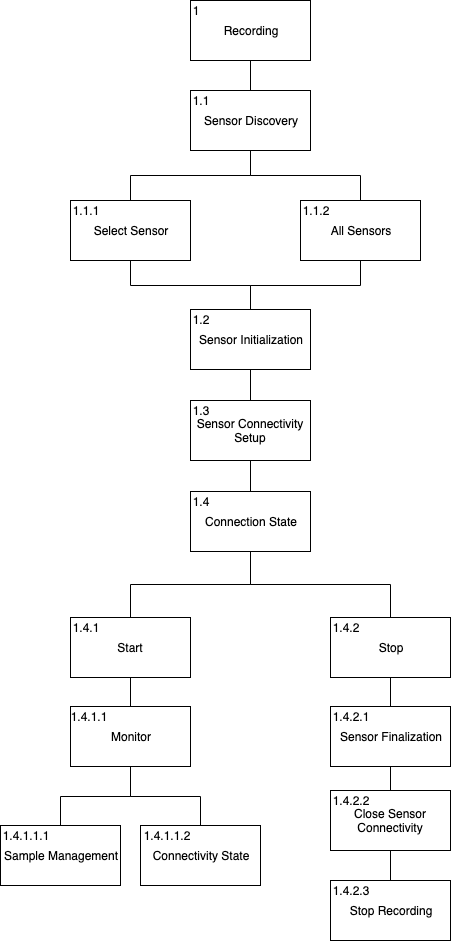
\includegraphics[width=0.65\textwidth]{images/Recording.png}
    \caption{Recording}
    \label{fig:hta_recording}
\end{figure}

\begin{itemize}
    \item Sensor Discover: Has to find all eligible sensors that can enable a recording.
    \item Select Sensors: From the sensor discovery, we can choose preferable sensors sources.
    \item  All Sensors: More straightforward, we sample from all of the available sensors.
    \item Sensor Initialization: Once we have a list of sensors sources, we need to establish and initialize a connection with the sensors. Occasionally a sensor might use some time to connect, or unforeseen occurrence is hindering the initialization of the sensor. Thus, blocking the state of the recording. 
    \item Sensor Connectivity Setup: Additionally, we establish a connection between the application and the sensor source. All data exchange occurs over the established interface. 
    \item Connection Stat: Based on sensors establishments we can proceed to either start or stop a recording. 
    \item Start: By starting, we notify the sensors to begin collecting data, and the view should display that a recording has begun accordingly.
    \item Monitor: Is continuously waiting for new samples to arrive on the interface defined between the application and the sensors.
    \item Sample Management: Once a new sample has arrived, we need to store the sample on a persistent storage.
    \item Connectivity State: If it is an external sensor, the sensor source might disconnect during a recording. Thus, implementing a mechanism to check for continuous data stream is a critical task.
    \item Stop: By stopping, we notify the sensors to stop collecting data from the sensor source.
    \item Sensor Finalization: We notify the sensor to stop sampling data, and close establishment.
    \item Close Sensor Connectivity: We close the interface establishment between the application and the sensors. 
    \item Stop Recording: Once the sensors has closed its connections, we can add additional information to the recording (e.g., title, description, rating). In the end, the recording has concluded and its stored on the mobile device.

\end{itemize}

This suggested structure of a recording is one alternative to enable a recording. Most of the components suggested in the structure are essential to a recording. A naive solution would be to ignore the connectivity state component, by assuming the sensors are connected indefinitely. In our thesis, we will be following 


\subsection{Sharing}

\subsection{Modules}

\subsection{Storage}

\subsection{Presentation}


\section{Data Structure}

\subsection{Data Formats} \label{sec:dataformat}

The data format is a part of the process of serialization, which enables data storage in a file, transmission over the Internet, and reconstruction in a different environment. Serialization is the process of converting the state of an object into a stream of bytes, which later can be deserialized by rebuilding the stream of bytes to the original object \cite{sumaray_comparison_2012}. There are several data serialization formats; however, JavaScript Object Notation (JSON) and eXtensible Markup Language (XML) are the two most common data serialization formats. This section discuss these formats, and in the end, we compare them and choose the format that meets the criteria of being compact, human-readable, and universal. 

\subsubsection{JSON}
JSON or JavaScript Object Notation is a light-weight and human-readable format that is commonly used for interchanging data on the web. The format is a text-based solution where the data structure is built on two structures: a collection of name-value pairs (known as objects) and ordered list of values (known as arrays). The JSON format is language-independent and the data structure universally recognized \cite{jsonorg, jsonvxml}. However, it is limited to a few predefined data types (i.e., string, number, boolean, object, array, and null), and extending the data type has to be done with the preliminary types. 

\begin{lstlisting}[language=json, caption={}, captionpos=b]
{
    "user": {
        "firstname": "Ola"
        "lastname": "Nordmann"
    }
}
\end{lstlisting}

\subsubsection{XML}
XML or eXtensible Markup Language is a simple and flexible format derived from Standard Generalized Markup Language (SGML), developed by the XML Working Group under the World Wide Web Consortium (W3C). An XML document consists of markups called tags, which are containers that describe and organize the enclosed data. The tag starts with \verb|<| and ends with \verb|>|; the content is placed between an opening tag and a closing tag. \cite{w3xml, jsonvxml} XML provides mechanisms to define custom data types, using existing data types as a starting point, making it extensible for future data. 

\begin{lstlisting}[language=json, caption={}, captionpos=b]
<user>
    <firstname>Ola</firstname>
    <lastname>Nordmann</lastname>
</user>
\end{lstlisting}

\subsubsection{Comparing}
With the study conducted by Saurabh and D’Souza \cite{jsonvxml}, we compare JSON and XML features and performance. There are apparent differences in the two data formats which affect the overall readability, extensibility, bandwidth performance, and ease of mapping. XML documents are easy to read, while JSON is obscure due to the parenthesis delimiters. XML allows for extended data types, while JSON is limited to a few data types. XML takes more bandwidth due to the metadata overhead, while JSON data is compact and use less amount of bandwidth.

Moreover, a few benchmarks were conducted to measure memory footprint and parsing runtime when serializing and deserializing JSON and XML data. From the conclusion,  in terms of memory footprint and parsing runtime, JSON performances better than XML, but at the cost of readability and flexibility. While these format structures are applicable for transmitting data, choosing a format that is compact, human-readable, and a standard format that is extensible and scalable for future data is essential. In our design, we use the JSON format for transmission of the data.

\begin{figure}
    \centering
    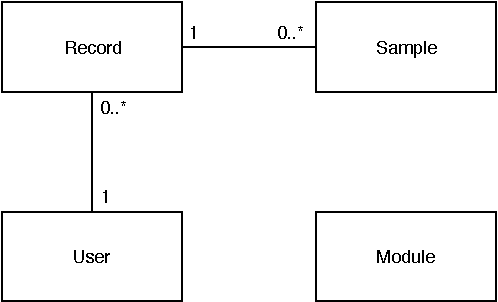
\includegraphics[scale=0.8]{images/DataEntries.pdf}
    \caption{The data model and relationship for the entities in the application: a record has zero to many samples, while a sample only can have one record. A record can have one user, while a user can have many records. A module has no relationship with the other entities.}
    \label{fig:dataentries}
\end{figure}

\subsection{Data Entities}\label{des:dataentity}
Data entities are objects (e.g., things, persons, or places) that the system models and stores information about. In Section \ref{soc:storage}, we introduced four data entities in the application (i.e., record, sample, module, and user). In Figure \ref{fig:dataentries}, the relations between the data entities are shown. The record entity and sample entity store information about the recording session\footnote{the ongoing process of collecting data from the sensor sources and storing the samples (data packets) in the database.} and are separated into two individual entities in order to reduce data redundancy and improve data integrity. The sample entity has a reference to its record entity so they can be associated with each other. The user entity store biometrical information related to the user (i.e., patients). Also, a record entity contains the state of the user's biometrical information at the time of the recording. In other words, the user's biometrical information can change over time (e.g.,  weight changes); therefore, capturing the exact biometrical information at the time of the recording is essential in the context of detecting sleeping illnesses with relation to the biometrical information.  A module entity is independent of the other data entities and stores information about the name and the package name of the module-application. The package name is used to locate and launch the module-application. 

In the following sections, we present the properties of each data entity in Nidra; storage structure of the entities, and illustration of the data structure for each entity.  



\subsubsection{Record Entity} \label{ssec:record}

The table for the record entity in the database stores metadata (e.g., elapsed time of recording, number of samples, user's biometrical data) related to a recording session. In Table 4.1, we present the information (fields) the record entity contains, which can be described as: 
\begin{itemize}
    \item \verb|ID|: Unique identification of a record, also a primary key for the entry.
    \item \verb|Name|: A name of the record to easily recognize the recording.
    \item \verb|Description|: A summary of the recording session provided by the user. It can be used to briefly describe how the recording session felt (e.g., any abnormalities during the sleep).
    \item \verb|MonitorTime|: The recording session duration in milliseconds.
    \item \verb|Rating|: Giving a rating on how the sleeping session felt, in a range between 0-5. 
    \item \verb|User|: User's biometrical information encoded into a JSON string format, in order to capture the state of the user at recording. 
    \item \verb|CreatedAt|: Date of creation of the recording in milliseconds (since January 1, 1970, 00:00:00 GMT).
    \item \verb|UpdatedAt|: Date of update of the recording in milliseconds (since January 1, 1970, 00:00:00 GMT).
\end{itemize}

\begin{table}[!h]
\begin{center}
\scalebox{0.75}{
\begin{tabular}{ |c|c|c|c|c|c|c|c| } 
\hline
\textbf{id} & \textbf{name} & \textbf{description} & \textbf{monitorTime} & \textbf{rating} & \textbf{user} & \textbf{createdAt} & \textbf{updatedAt} \\
\hline
1 & Record \#1 & - & 5963088 & 2.5 & \{...\} & 1554406256000 & 1554406256000  \\ 
\hline
\end{tabular}}
\caption{Example entry in the record table.}
\end{center}
\end{table}





\subsubsection{Sample Entity} \label{ssec:sample}
The table for the sample entity contains a single sensor reading (data packet) sent from the sensor source. Sample entity are stored separated from a record entity; however, they are linked (foreign key) with their corresponding record entity. In Table 4.2, we present the information (fields) the sample entity contains, which can be described as: 

\begin{itemize}
    \item \verb|ID|: Unique identification of a sample, also a primary key for the entry.
    \item \verb|RecordID|: An identification to its corresponding record, also a foreign key. 
    \item \verb|ExplicitTS|: Timestamp of sample arrival based on the time in the sensor. 
    \item \verb|ImplicitTS|: Timestamp of sample arrival based on the time on the device. 
    \item \verb|Sample|: Sensor reading contains metadata and data according to Flow sensor.
\end{itemize}

\begin{table}[!h]
\begin{center}
\scalebox{0.60}{
\begin{tabular}{ |c|c|c|c|c| } 
\hline
\textbf{id} & \textbf{recordId} & \textbf{explicitTS} & \textbf{implicitTS} & \textbf{sample} \\
\hline
1 & 1 & 1554393086000 & 1554400286000 & Time=0ms, deltaT=100, data=1906,1891,1884,1881,1876,1718,1690 \\ 
\hline
\end{tabular}}
\caption{Example entry in the sample table.}
\end{center}
\end{table}



\subsubsection{Module Entity} \label{ssec:module}
The table for the module entity contains metadata of the module added by the user in the application. In Table 4.3, we present the information (fields) the module entity contains, which can be described as:
\begin{itemize}
    \item \verb|ID|: Unique identification of a module, also a primary key for the entry.
    \item \verb|Name|: The name of the module-application.
    \item \verb|PackageName|: The package name of the module-application, such that it can be launched from Nidra. 
\end{itemize}

\begin{table}[!h]
\begin{center}
\scalebox{0.8}{
\begin{tabular}{ |c|c|c| } 
\hline
\textbf{id} & \textbf{name} & \textbf{packageName} \\
\hline
1 & OSA Predicter & com.package.osa\_predicter \\ 
\hline
\end{tabular}}
\caption{Example entry in the module table.}
\end{center}
\end{table}


\subsubsection{User Entity} \label{ssec:user}
The user of the application is the patient, which provides biometrical data (e.g., weight, height, and age). The biometrical data is part of the application to enrich the record. The record captures the biometrical state of the user at the time of the recording. In Nidra, the user entity is not a part of the database, but stored as an object on the mobile device. The design decision of this choice is because the application is limited to one user at the time, and it makes it convenient to capture the state of the object of the given time of recording. It is possible to create a table in the database for the user entity, and for each time the user changes the biometrical data insert it is a separate entry in the database. The record could then have a reference to the latest user entry. However, that increases the complexity of the system, and as of now, the design of the application is to store the user's biometrical data into an object on the device. 

In the listing below, we present the structure of the user entity. In Nidra, the user entity is stored as an object and structured as a JSON format containing biometrical data related to the user: 
\begin{itemize}
    \item \verb|Name|: A string that contains the name of of the patient.
    \item \verb|Age|: An integer with the age of the patient.
    \item \verb|Gender|: A string that contains the gender of the patient.
    \item \verb|Weight|: An integer with the weight of the patient in kilograms.
    \item \verb|Height|: An integer with the height of the patient in centimeters.
\end{itemize}

\begin{figure}[!h]
\begin{lstlisting}[language=json, caption={}, captionpos=b]
{
    "user": {
        "name": "Ola Nordmann",
        "age": 50,
        "gender": "Male",
        "height": 180,
        "weight: 60
    }
}
\end{lstlisting}
\end{figure}



\subsection{Data Packets}\label{design:datapackets}
Data packets are parcels of data that Nidra receives from external applications (e.g., data streams dispatching module) or send to other application (e.g., by sharing the records on the device). This section presents the format of the records and corresponding samples that are sent across applications (e.g., the data is encoded into a file, and the user can select preferred media, such as e-mail), and presents the data packets forwarded by the data streams dispatching module upon data acquisition from the Flow sensor.

\subsubsection{Sharing}

In \Cref{sec:design_sharing}, a proposal for the structure of exporting and importing data is discussed. Two of the components (\verb|Parse Formatted Content| and \verb|Format File|) use JSON to either encode or decode the data. Listing 4.1 illustrates the content of the encoded data from the application to gain a broader understanding of how the data format looks. To summarize, the JSON string contains an object of record that encompasses the metadata of the recording session, as well as the state of biometrical data of the user. Besides the record object, there is an array of sample objects, where each sample object contains a single sensor reading from the Flow sensor. 

\begin{lstlisting}[language=json, caption={A JSON string object that contains the record which has metadata from the recording session (including the biometrical data of the user), and a list of samples (where each samples contains a single sensor reading).}, captionpos=b]
{
    "record":{  
        "id": 1,
        "name": "Record 1",
        "rating": 2.5,
        "description": "",
        "nrSamples": 6107,
        "monitorTime": 5963088,
        "createdAt": "Apr 4, 2019 9:30:56 PM",
        "updatedAt": "Apr 4, 2019 9:30:56 PM",
        "user": {  
            "age": 50,
            "createdAt": "---",
            "gender": "Male",
            "height": 180,
            "name": "Ola Nordmann",
            "weight": 60
        }
    },
    "samples": [  
        {  
            "explicitTS":"Apr 4, 2019 5:51:26 PM",
            "implicitTS":"Apr 4, 2019 7:51:26 PM",
            "recordId":1,
            "sample":"Time=0ms, deltaT=100, data=1906,1891,1884,1881,1876,1718,1690"
        },
        ...
    ]
}
\end{lstlisting}

\subsubsection{Single Sensor Reading}

Listing 4.2 presents a single sensor reading from the Flow sensor sent from the data streams dispatching module. The \verb|id| is assigned by the data streams dispatching module to identify the subscriber application with the corresponding sensor source. Moreover, the \verb|time| is assigned by the internal timer of the Flow sensor. Also, the \verb|value| is the data sent from the Flow sensor, which encompasses time, delta, and data. However, we are most interested in extracting the data values from the reading. 

\begin{lstlisting}[language=json, caption={Encompasses a single sample received from the Flow sensor.}, captionpos=b]
{
    "id":"1-0",
    "value":"Time=2100ms, deltaT=100, data=1869,1873,1883,1864,1871,1870,1870",
    "time":"2019-07-29T18:20:58.997+0000"
}
\end{lstlisting}


